%%==========================
%% chapter01.tex for TJU Master Thesis
%% based on CASthesis
%% modified by charlie.yaha@gmail.com
%% version: 0.1alpha
%% Encoding: UTF-8
%% last update: Dec 5th, 2010
%%==================================================

%\bibliographystyle{TJU} %[此处用于每章都生产参考文献]


\newcommand{\citeA}[2]{\citeauthor{#1}\cite{#1}}

\chapter{绪~论}

\section{研究背景及意义}
地下介质普遍具有非弹性衰减性质,其衰减性通常用品质因子$Q$来表征。
地震尺度内的非弹性衰减主要是与介质内部介关尺度(介于波长与颗粒尺度之间)的
弹性非均匀性或流体饱和非均匀性诱导的波致流体流现象有关
(\citeA{pride:2003},\citeA{muller:2010})。
地震波衰减对地表观测数据有非常重要的影响,
主要表现在如下两方面:首先,衰减会减弱地震波的振幅;其次,衰减改造地震波相位以致
速度频散。图(\ref{fig:spectral}a)对比了在同一时刻接收的
非衰减介质中的地震波(蓝色)和在$Q=60$的粘声介质中传播的地震波的波形。可以看出,衰减介质中传播地震波
的振幅被极大程度地吸收衰减。由于地震波衰减导致速度频散,高频成分具有更快的传播速度,所以
不同频率成分具有不同的到达时。
图(\ref{fig:spectral}b)对应地展示了图(\ref{fig:spectral}a)中两种波形的振幅谱。
从图中可以看出,高频成分的衰减要
远远严重于低频成分,这也是造成图(\ref{fig:spectral}a)中振幅强衰减的主要原因。

\begin{figure*}[!htbp]
        \centering
		\subfigure[]{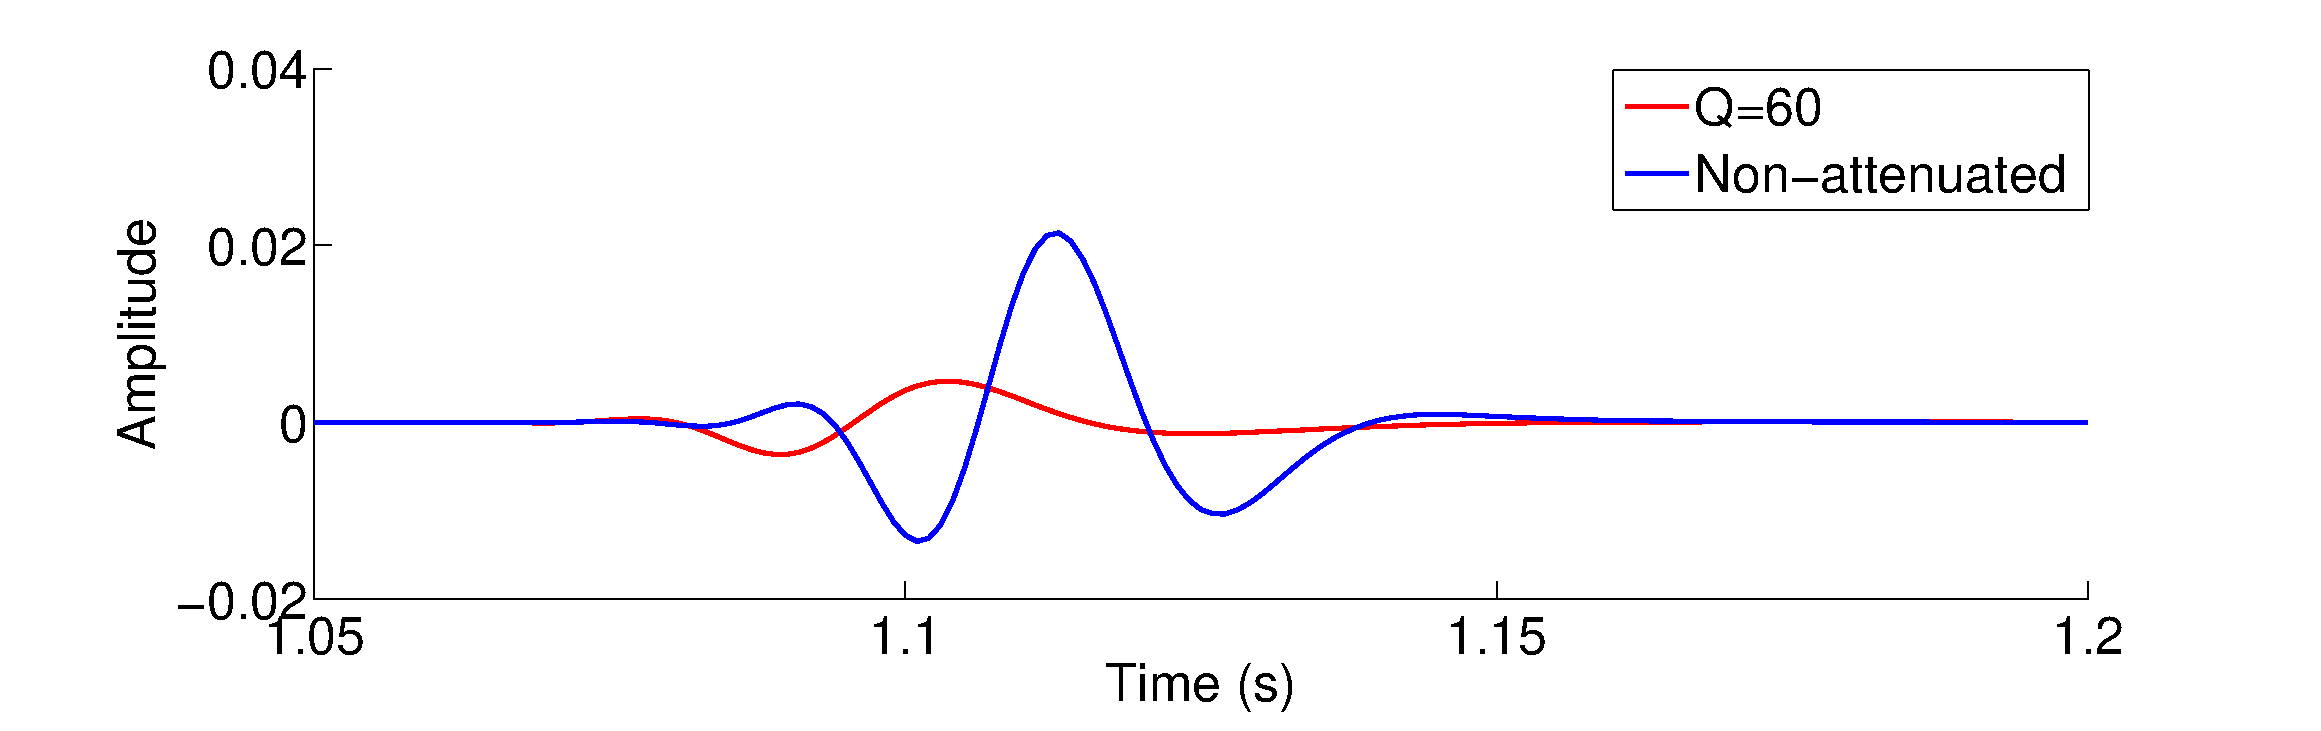
\includegraphics[width=0.9\linewidth]{figure/wavelet_ch1}}
		\subfigure[]{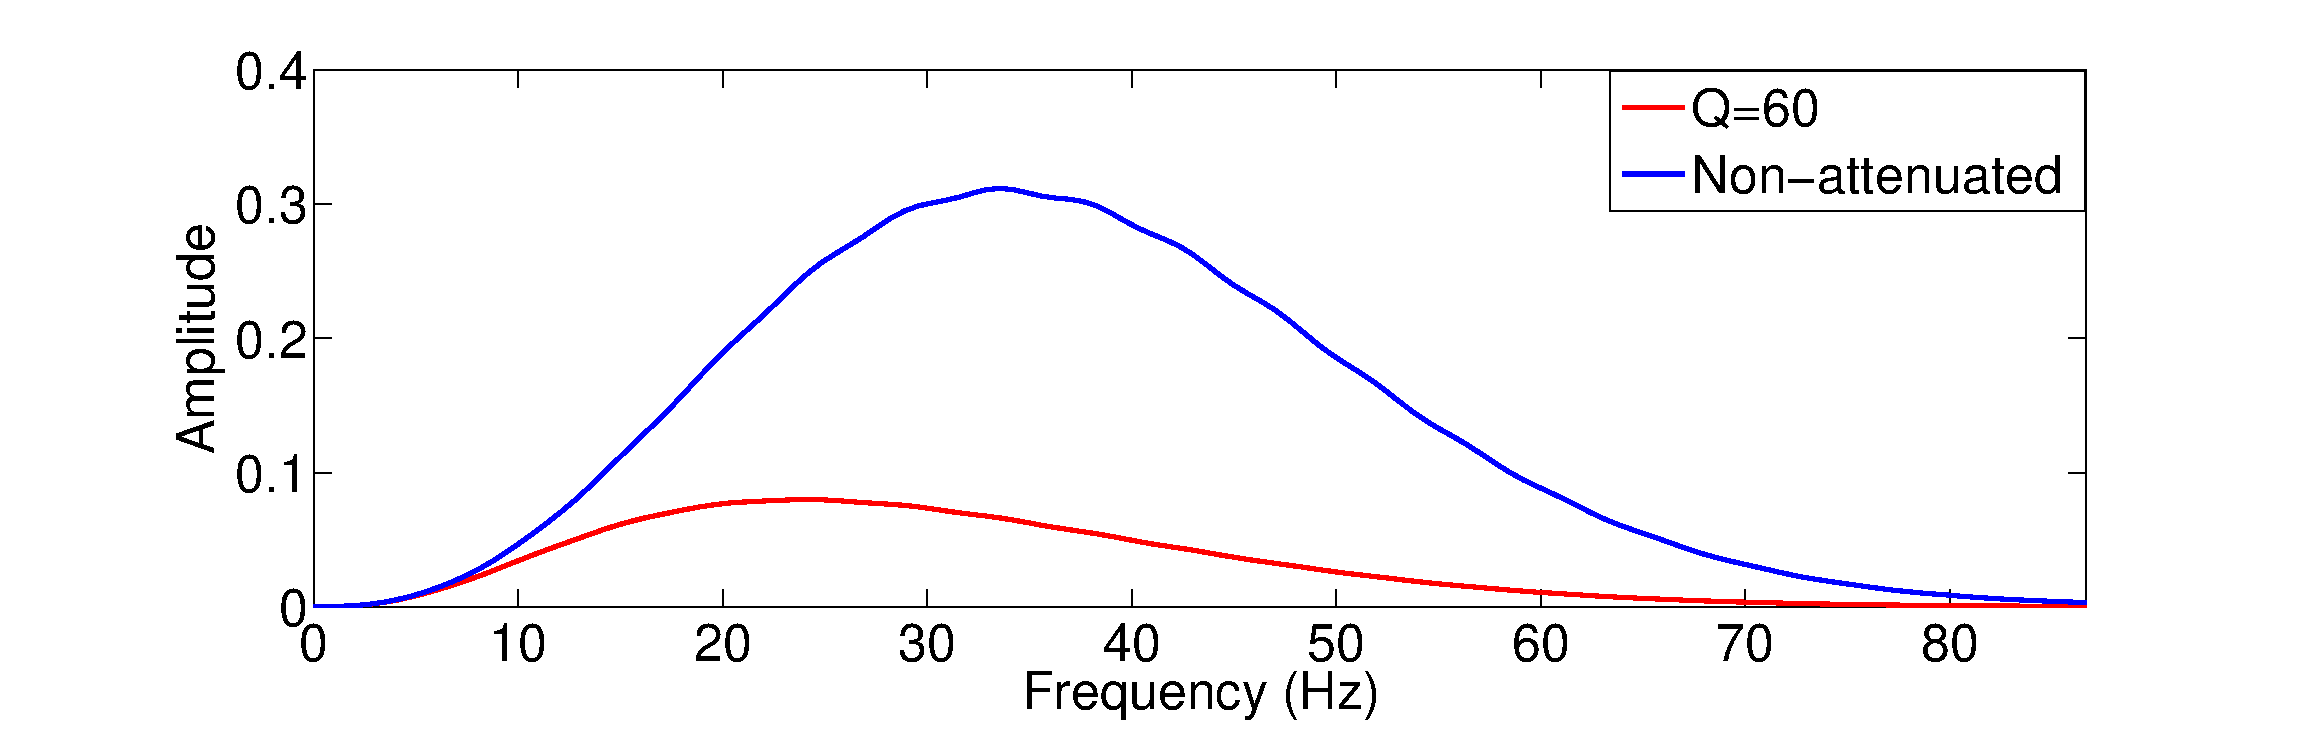
\includegraphics[width=0.9\linewidth]{figure/spectrum_ch1}}
        \fcaption{地震波在声介质和粘声介质($Q=60$)中传播的数值模拟实验:
	(a)地震波波形图;(b)对应的振幅谱。}{1D example to numerically illustrate the attenuation 
	impacts on the amplitudes spectra and phase of propagating wave: (a) the 
	non-attenuated waveform (blue curve) and the attenuated waveform (red curve); (b) the 
	corresponding amplitude spectral. }[展示地震衰减效应的一维数值实验]
        \label{fig:spectral}
\end{figure*}

非弹性衰减通过吸收地震波的
高频成分和改造地震波的相位来降低地震波成像的分辨率。在地震波偏移成像中,
如果不补偿$Q$的效应会影响地震成像的质量进而影响后续的地震解释和储层识别。
图(\ref{fig:qrtm_1}a)展示了墨西哥湾某工区常规
逆时偏移(RTM)成像结果,图(\ref{fig:qrtm_1}b)对应地展示了用$Q$补偿的逆时偏移($Q$-RTM)
成像结果(\citeA{zhang.zhang:2010})。由于强衰减的影响,使得常规RTM在衰减区域及其下方成像模糊,
通过$Q$补偿使得整个成像剖面的振幅更加均衡,且很好地恢复了由衰减引起的成像阴影区的地层信息。

\begin{figure*}[!htbp]
        \centering
		\subfigure[]{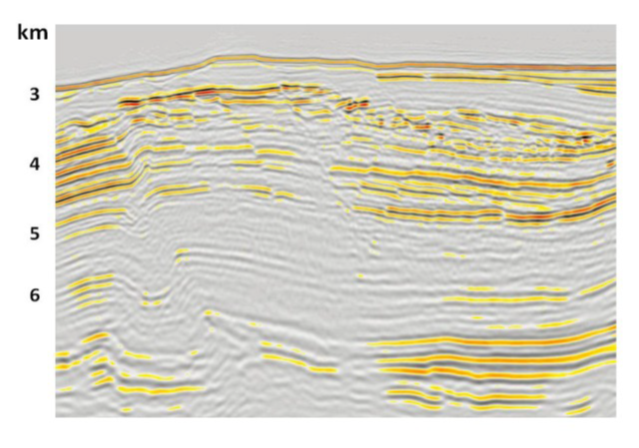
\includegraphics[width=0.495\linewidth]{figure/mig_no_ch1}}
		\subfigure[]{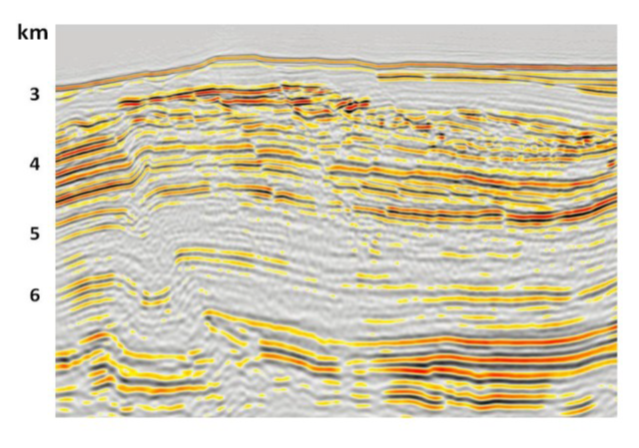
\includegraphics[width=0.495\linewidth]{figure/mig_q_ch1}}
		\fcaption{衰减对地震成像的影响:(a) 传统RTM成像结果;(b)$Q$-RTM成像结果
		(\citeA{zhang.zhang:2010})。
		}{A comparison of conventional RTM (a) and $Q$-RTM (b) results..
		}[衰减对地震成像的影响]
        \label{fig:qrtm_1}
\end{figure*}

在实际勘探中,气云区的地震成像、解释和储层识别都面临巨大的挑战。气云区通常包含极低的
$Q$值,强烈的衰减会吸收深部反射波的能量,在储层的上方造成成像阴影区,严重影响地震
解释的准确性。可靠的$Q$模型不仅可以提高成像的质量,而且可以更好解释振幅随偏移距变化
(AVO)和各向异性这两种依赖于偏移距的效应。正确的AVO和各向异性
解释可以提高油气勘探的成功率。另外,$Q$模型可以作为一个表征岩石和流体属性的参数。
例如,在稀疏井约束下可以用$Q$值来检测岩性的边界(\citeA{desgupta.clark:1998})。
衰减系数是一个直接刻画储层的油气物理参数,例如可以利用$Q$模型来确定储层含油/气
的饱和度(\citeA{winkler.nur:1982})。在油气开发过程中,衰减模型还可以用来指示储层裂缝的方位
(\citeA{maultzsch.chapman:2007}; \citeA{clark.benson:2009}),也可监控流体的运移能力,
帮助优化注水过程(\citeA{macrides.kanasewich:1987})。
因此,在油气勘探开发过程中,定量地评估非弹性衰减效应,构建一个可靠的本征衰减($Q$)模型是非常重要的。
鉴于地震波非弹性衰减的路径效应比界面影响更大,
本文主要的工作就是通过反射波形反演来定量估计宏观的地震本征衰减$Q$模型。

\vspace{1.2cm}
\section{国内外研究现状}
\vspace{0.4cm}

国内外学者对$Q$模型估计开展了大量的研究,其中大部分工作都是数据域的分析和反演方法。数据域的
$Q$反演方法可大致分为两类:基于高频近似的射线层析类和基于波动方程的波形反演类。

在射线类层析方法中,\citeB{brzostowski.mcmechan:1992}首先用观测数据振幅与震源振幅比值的对数作为输入数据来
实现$Q$层析成像。除了吸收衰减外,影响振幅的因素还有很多,如几何扩散、透射/反射损失、
散射损失等。为了区分衰减引起的振幅损失,\citeB{quan.harris:1997}将观测数据和计算数据之间质心
频率的移动作为匹配依据,用射线层析来更新$Q$模型。\citeB{hu.liu:2011}用震源的振幅谱作为
拟合函数来处理地震数据频谱非对称性的影响,并用多指数盒状约束法来消除非地震本征衰减的影响。
质心频率移动类的方法相对于振幅匹配类方法对噪音不敏感,更适合处理实际地震数据。
射线类方法计算效率高,处理横向变化缓慢的介质有很好的效果。当上覆介质横向非均匀性很强时,
地震波存在多路径,射线类方法由于不能有效处理多路径效应而造成误差。波动方程层析方法可以
有效的解决多路径问题,从而提高反演的分辨率。

全波形反演(FWI)是一种通过求解波动方程来恢复地下介质参数的反演迭代方法(\citeA{tarantola:1984})。
FWI是一个高度非线性的反演问题(\citeA{mora:1987};\citeA{sirgue.pratt:2004}),需要
大量的波场正演计算,全局寻优的解法(\citeA{sen.stoffa:1991};\citeA{mosegaard.tarantola:1995})
所需的计算量仍是现在计算机所不能承受的。伴随状态法的引入(\citeA{lailly:1983};
\citeA{tarantola:1984};\citeA{pratt.worthington:1990})使得目标函数梯度的计算变得非常高效,目前基于
梯度类的解法已趋于成熟。在勘探地震学中,各种应用实例证明粘声波形反演($Q$-FWI)对于提供高
分辨率的P波速度结构有非常重要的作用(\citeA{song:1995};\citeA{ravaut:2004} 
;\citeA{gao:2006}; \citeA{kamei:2012})。由于衰减参数相较于速度参数对目标函数
的影响更弱且这两种参数之间还存在强烈的耦合性(trade off),衰减参数的波形反演比速度的波形反演更具挑战性(
\citeA{song:1995};\citeA{liao.mcmechan:1996};\citeA{smithyman:2009};\citeA{hak.mulder:2011} 
;\citeA{malinowski:2011};\citeA{bai:2014};\citeA{kamei.pratt:2013})。

\citeB{tarantola:1988}在时间域粘弹波形反演理论中首次考虑了衰减参数的波形反演。
随后,\citeB{song:1995}在频率域提出了一种粘声波形反演方法。在频率域实现波形反演比时间域
有如下优势,尤其是考虑衰减效应: 首先,衰减参数(例如$Q$值)和频散速度关系很容易用随频率
变化的复速度来表示,目标函数对速度和衰减参数的梯度可以同时得到而不需要额外的计算量(\citeA{song:1995})。
另外,频率域反演方法可以自然的实现多尺度反演策略以降低波形反演的非线性(\citeA{bunks:1995};
\citeA{sirgue.pratt:2004})。从最低的频率成分开始反演,并逐渐增加高频成分,这样可以
逐渐重建高分辨率的地下速度和衰减模型。

在波形反演中,速度和衰减参数$Q$有很强的耦合性(\citeA{song:1995};\citeA{kamei.pratt:2008};
\citeA{hak.mulder:2011})。\citeB{ribodetti:2000}以及\citeB{hak.mulder:2010}讨论了观测系统的
重要性。他们指出,完美的地下照明可以解决这种参数串扰问题。\citeB{innanen.weglein:2007}用逆散射
理论和一阶的频散反射系数来区分一维速度和衰减系数结构。\citeB{mulder.hak:2009}调查了
线性Born反演的零空间情况,并且指出,在计算梯度时如果不考虑速度频散关系,对于给定的地表反射数据,
地下许多速度/衰减对存在无解的情况。\citeB{hak.mulder:2011}指出,对于地表观测系统,考虑了频散关系
的非线性波形反演可以较精确地反演简单二维理论模型的速度和衰减系数。
然而,在早些阶段的反演中,串扰现象还是很明显,并且需要非常多(在他们的实验中大于10000次)的迭代
次数来消除,因此该反演问题还是非常病态的。此外,由于参数间强耦合性的影响,
考虑纵横波速度、密度、衰减参数的弹性波形反演
(\citeA{yang:2017},\citeA{fabien:2017})更有挑战。

在$Q$-FWI中,各种各样的预条件方法被用来减弱反演的病态性。\citeB{liao.mcmechan:1996}用合成数据
实验显示要获得好的衰减模型,必须要对模型参数进行一定的范围约束。\citeB{hak.mulder:2011}指出
基于两种参数特征值的大小来惩罚梯度中衰减成分可以加速$Q$-FWI的收敛。\citeB{malinowski:2011}
在波兰某盆地成功地反演出了与岩性信息一致的衰减模型。他们指出对地震数据时间方向强阻尼衰减
和梯度大尺度平滑约束是反演$Q$参数的关键。

对于$Q$反演的另一类做法是顺序反演,即先获取比较准确的速度模型然后再反演$Q$模型。如果我们认为
反演前期的振幅变化主要是由于速度结构引起的,后续再反演$Q$时可以降低参数间的串扰。初始的速度估计是通过
固定初始衰减模型来反演(\citeA{pratt:2004};\citeA{kamei.pratt:2008};\citeA{rao.wang:2008};
\citeA{smithyman:2009})。\citeB{pratt:2004}用顺序反演法处理含碳氢化合物的强衰减跨井数据。
对于$Q$模型的反演,他们也用了较大的平滑约束,其反演结果与超声波形分析结果有很好的一致性。
\citeB{watanabe:2004}在超声频段用实验室数据同样很好实现了顺序反演方法。\citeB{smithyman:2009}
用顺序反演法来识别近地表非弹性衰减目标体。\citeB{watanabe:2004}以及\citeB{kamei.pratt:2008}用合成跨井数据
比对了同时反演和顺序反演的结果,发现在没有正则化项的情况下,顺序反演会得到更好的结果。
\citeB{kamei.pratt:2008}认为地震数据中大部分振幅变化是由速度变化引起的。
\citeB{kamei.pratt:2013}系统地调查了不同梯度预条件对$Q$反演的影响。

地震数据的走时信息主要受速度参数影响,地震衰减通过速度频散影响走时,但衰减的振幅效应
更明显。相较于走时信息,地震振幅很容易受噪音、震源检波器的耦合、震源的辐射模式以及
弹性(非声学)效应的影响。为了保证振幅信息的准确性,需要非常细心的前处理工作(\citeA{pratt:2004};
\citeA{malinowski:2011})。\citeB{dutta.schuster:2016}通过将峰值频率移动引入到$Q$-FWI中
来降低数据对前处理的依赖,从目标函数出发降低了$Q$-FWI的非线性程度。

FWI需要低频、全方位、大孔徑地震数据,但是这种高质量的数据采集往往需要高昂的代价。
通过不同观测孔径的观测系统照明分析可知,当缺少大孔径的回转波或折射波数据时,深部模型往往只被
反射波照明。因此,利用反射波进行中深部的速度建模已成为共识。
当反射数据占主导时,常规FWI的梯度中高频成分占主导,反射波的偏移响应与利用反射波反演
背景模型的核函数相比,数值上往往高一个数量级,因此,常规FWI只会得到一个
高波数的成像结果,不易于更新背景模型(\citeA{wu.alkhalifah:2014};\citeA{alkhalifah:2015};
\citeA{chi:2015};\citeA{alkhalifah.wu:2016})。
为改善对模型低频成分的更新,学者们提出了梯度预条件方法(\citeA{Liu:2011};\citeA{wang:2013};
\citeA{tang:2013}),目的是增强层析分量的贡献进而得到有效的低波数模型的更新。
为了解决反射波数据占主导情况下FWI的上述问题,\citeB{xu:2012a}提出了反射波形反演
方法(RWI)。其思想在于:将速度模型分解为背景模型和扰动模型两部分,利用反射波数据侧重更新
背景速度而非高波数的速度扰动。

但是,为了使RWI能够在实际地震资料反演中更好地恢复中深层背景速度,需要进行数据匹配和反射系数估计
(真振幅成像)。\citeB{ma.hale:2013}利用DIW算法(Dynamic image warping)提取反射波的走时时差,
实现中深层背景速度建模,提高反演的稳定性。\citeB{alkhalifah:2016}用散射角滤波的全模型反演方法
来解决数据分级匹配问题。基于相关的反射波形反演方法(\citeA{chi:2015}),在一定程度上也避免了
数据匹配的周期跳跃问题。即使在观测数据中缺乏有效低频信息、背景模型相对较差时,RWI也可以较好地
恢复模型中深部的低波数成分。在反射系数估计方面,最小二乘偏移(\citeA{dai.schuster:2013};
\citeA{zhang:2014})是目前比较有效的方法。但是,最小二乘偏移要求背景模型要足够准确
(\citeA{luo.hale:2014}),否则其反演的高波数模型扰动也不正确,而这又与
RWI反演背景速度的目标相矛盾。因此,在反射波波形反演中,如何以及何时引入最小二乘偏移将显得非常重要。
最近,\citeB{cheng:2018}提出了基于模型尺度分解,P/S波模式解耦的反射走时与波形反演方法,
交替更新纵横波速度的宏观背景与高波数扰动。这项工作对基于反射波的多参数反演有一定的借鉴意义。

此外,\citeB{shen.biondi:2018}在成像域建立起了模型扰动与偏移图像扰动的关系,
通过$Q$偏移分析估计中深层的背景$Q$模型。
目前还没人探讨用地表反射地震数据恢复中深层背景$Q$模型的数据域反演方法。
本文将研究如何把RWI引入到背景$Q$反演中。

\vspace{0.9cm}
\section{本文研究内容}
\vspace{0.5cm}

本征衰减参数$Q$对地震波振幅的影响类似于速度对走时信息的影响,是一种沿地震波路径累积叠加的效应,
并且主要受$Q$模型的低波数(背景)成分控制。在实际应用中,相对准确的背景$Q$模型即可补偿成像中
能量的损失和相位畸变,提高成像分辨率。本文结合地震衰减的具体特点,在RWI的框架下
,实现中深层背景衰减模型的反演。具体研究内容包括:

在第二章中,首先简单回顾了地震衰减的基本理论,分析表征地震衰减的物理参数(品质因子和吸收系数);
其次系统地总结了描述地震衰减的不同本构关系模型,并重点回顾了勘探地震学中常用的两类模型(标准线性固体模型
和常$Q$模型);然后推导了描述这两类衰减模型的粘声波方程,并比较了这两种方程波场模拟的结果;最后
总结了$Q$-RTM所遇到的问题及其解决办法,并比较了上述两类方程在$Q$偏移
成像中的应用。

在第三章中,在顺序反演的思路下,提出了宏观衰减模型反射波形反演($Q$-RWI)方法。
先假定速度模型准确,将速度分解为背景和扰动两部分,基于标准线性固体模型粘声波方程
通过Born正演实现反射波模拟。在RWI的框架下,用波形数据残差作为
目标函数来更新中深层背景$Q$模型。

在第四章中,首先讨论了反射地震数据的峰值频率属性与速度高波数模型的关系;其次用峰值频率
移动目标函数来降低$Q$-RWI对高波数速度模型的依赖;然后用短时傅里叶变换(STFT)
提取多反射震相数据的峰值频率;最后通过数值实验验证峰值频率移动目标函数
的可靠性。


最后,总结论文的主要结论和创新点,并讨论不足之处以及未来的研究方向。

















